\chapter{Alkalmazás és hardver fejlesztése}

Ebben a fejezetben bemutatom az eddig elvégzett feladatokat és ezzel együtt a fejlesztés általános folyamatát is egy ilyen heterogén rendszerre. A fejlesztés ilyen rendszerekre közel sem triviális, szerencsére a gyártó általában ad valamilyen kiindulási pontot a kezdéshez, ez a Xilinx esetében is igaz.
\cite{Tutorial}

\section{Vivado base platform}
Ebben a részben a fejlesztés első lépése kerül bemutatásra. A Vivado base platform egyfajta alapot vagy keretet ad az egész projektnek. Ennek a lépésnek a végén rendelkezésre kell állnia egy .xsa fájlnak, ami olyan információkat tartalmaz a hardverről, amiket a fejlesztés további lépéseiben feltétlenül ismerni kell.

\subsection{A base platform részei}
A base platformot a Xilinx Vivado fejlesztő környezet segítségével hoztam létre. Ezen belül a blokkvázlat készítő funkciót kellett használni, amihez sok esetben az IP integrator-ral kellett blokkokat hozzáadni. Az így elkészült blokkvázlatot lehet .xsa fájlként exportálni.

\subsubsection{Zynq MPSoC blokk}
A Vivado base platform talán legfontosabb része a Zynq UltraScale+ MPSoC blokk. Ezt a blokkot készen hozzá tudjuk adni a blokkvázlathoz az IP integrátor segítségével. Hozzáadás után a blokk alapértelmezett beállításokkal kerül hozzáadásra. Az alapértelmezett beállítások függenek a kártya típusától, ezt értelem szerűen a projekt kezdetén be kellett állítani. Az alapértelmezett paramétereket lehet szabadon módosítani, ez saját tervezésű PCB-k esetében lehet érdekes, itt nincs ilyen módosításokra szükség.

Ez a blokk tartalmazza a PS konfigurációit és pin kiosztását. Ez a blokk szolgáltat információt arról, hogy hogyan tudjuk majd PL-ban megtervezett hardvert elérni a PS irányából.

\begin{figure}[!ht]
    \centering
    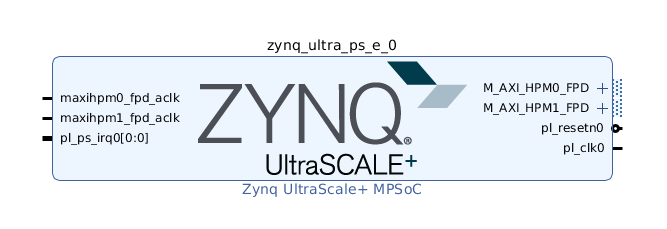
\includegraphics[width=150mm, keepaspectratio]{figures/block_automation_result.png}
    \caption{Zynq UltraScale+ MPSoC blokk}
\end{figure}

\subsubsection{Órajelek}
Órajelek előállítására rendelkezésre áll a Clocking Wizard nevű IP. Az IP blokk konfigurációja egyszerű, csak meg kell adni, hogy melyik órajelet milyen frekvencián szeretnénk, és az IP elrejti a hardver leírását.

Ebben a feladatban 3 különböző órajelet csinálunk. A rendelkezésre álló órajelek frekvenciái: 100 MHz, 200 MHz és 400 MHz. Ezek közül a későbbiekben bemutatásra kerülő V++ linker a teljes design előállításánál intelligensen tud majd választani. Referencia órajelnek a \mycode{pl\_clk0} nevű órajelet használjuk. Ez a jel a PS felől érkezik, így a blokkvázlaton a Zynq UltraScale+ MPSoC blokk kimeneti jeleként szerepel.

\subsubsection{Reset jelek}
A hardver reset szükségleteinek ellátására is rendelkezésünkre áll egy IP blokk. Mindhárom előállított órajelhez szükség van egy reset jelre is, így három darab Processor System Reset nevű blokkra lesz szükségünk. A három reset blokknak különbözőek az órajelei, de az external reset bemenetük ugyanarra a PS felől érkező reset jelre (\mycode{zynq\_ultra\_ps\_e\_0/pl\_resetn0}) van kötve.

\subsubsection{AXI interface}
A PS és a PL a Xilinx heterogén rendszereiben általában AXI busz interfészen tud kommunikálni. Az IP integrator segítségével hozzá kell adnunk a design-hoz egy AXI Interrupt Controller nevű IP blokkot. 

Ennek a blokknak a konfigurálása során létrehozunk a PS irányából master-nek számító AXI GP (General Purpose) interface-eket. Ezeken keresztül tud majd a szoftver kommunikálni a PL-kal. Ezen kívül a V++ linker automatikusan létrehoz további ilyen irányú AXI interface-eket amiken keresztül a szoftver fel tudja használni a rendelkezésre álló hardveres gyorsító-erőforrásokat.

Szükség van másik irányú kapcsolatra is, tehát a PS-nek slave-ként is kell viselkednie. Ezeken az interface-eken a hardveres gyorsítók a PS-hez tartozó RAM-ot tudják majd elérni.

\subsection{Exportálás}
A base platform már tulajdonképpen készen van, azonban minden hardver design-hoz szükség van egy top modulra. Ezt jelen esetben HDL wrapper-nek hívják, és a Vivado automatikusan le tudja generálni.\\

\begin{figure}[!ht]
    \centering
    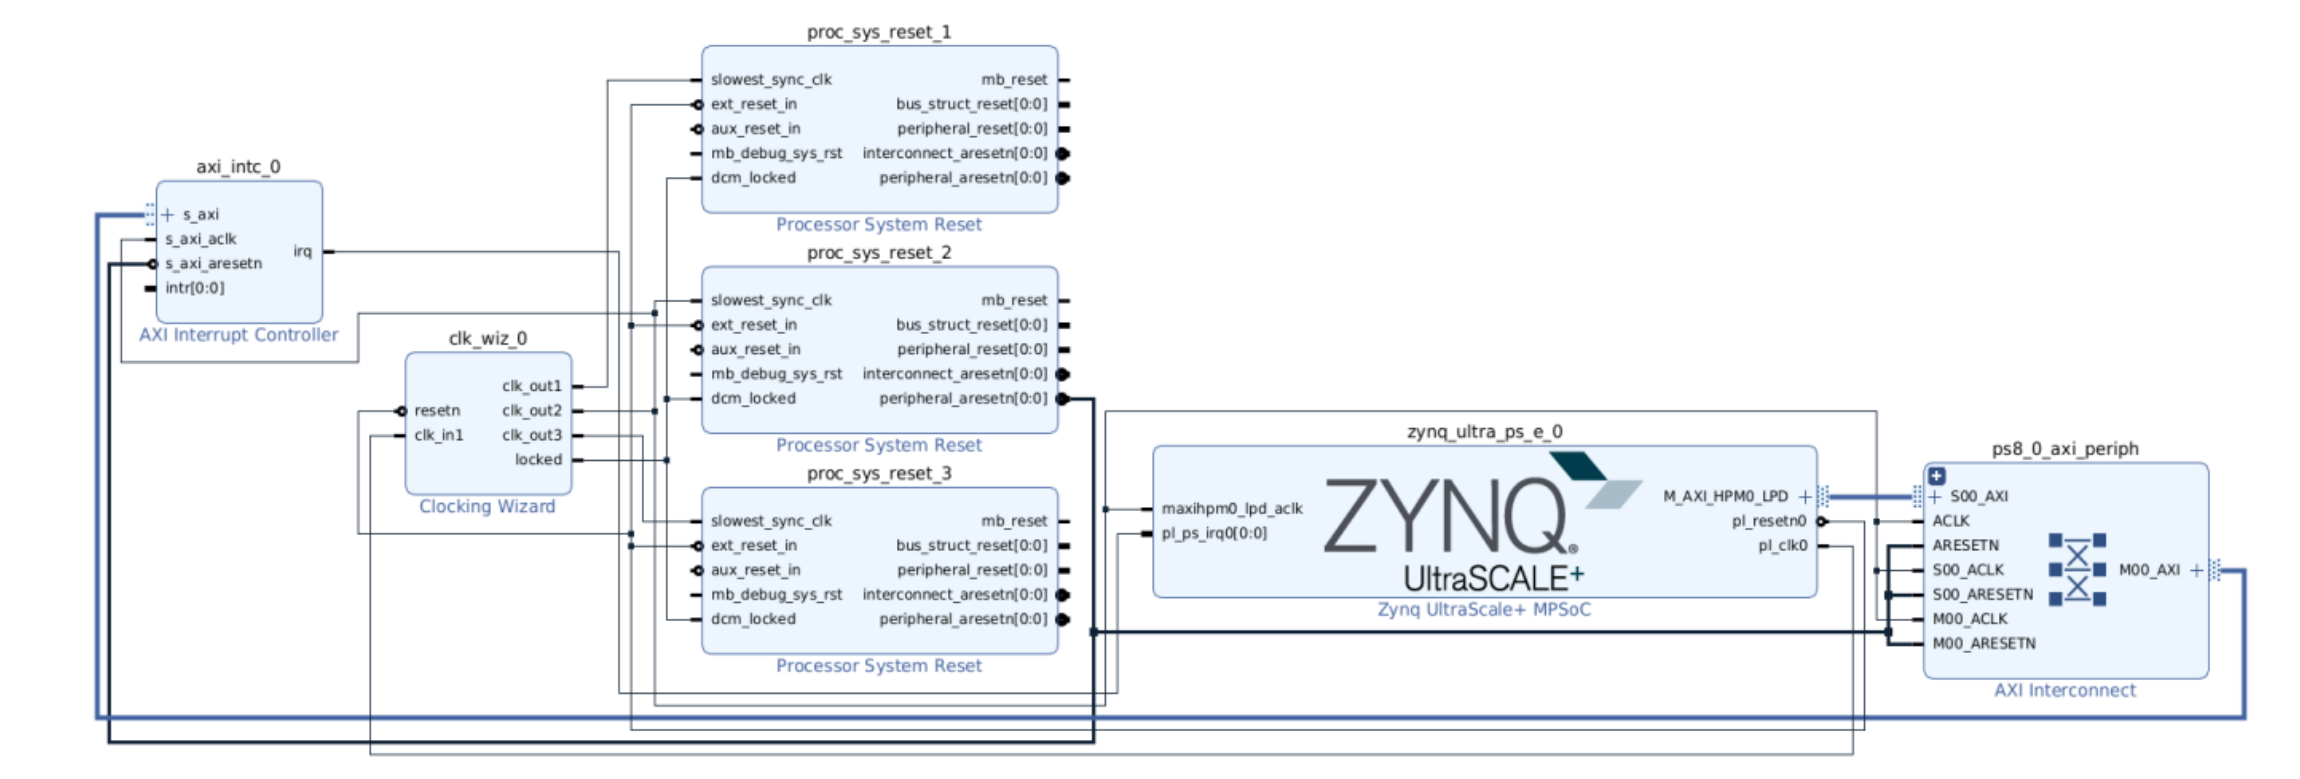
\includegraphics[width=150mm, keepaspectratio]{figures/base_platform.png}
    \caption{A teljes Vivado base platform}
\end{figure}

A Generate Block Design fázis választása után lehet exportálni az elkészült pre-synthesis design-t az Export Platform opcióval. Az elkészült design-hoz lehetőség van bitstream-et is generálni, erre azonban a feladat során nincs szükség. Az elkészült .xsa fájlt a következő lépesek bemeneteként fogjuk felhasználni, és a PL konfigurációja a fejlesztés során egy későbbi lépésben fog elkészülni.

\section{Software platform - Petalinux}
Ebben a fejezetben a már említett Arm CPU magokon futó szoftver platform kerül bemutatásra. A Xilinx heterogén rendszerek PS részén futó operációs rendszer a Linux egy erre a célra kifejlesztett fork-ja, a Petalinux.

\subsection{Alaptulajdonságok}
A Petalinux egy hardver specifikus szoftver környezet. Ez alatt azt kell érteni, hogy az operációs rendszer összetétele, leginkább a device tree-hez kapcsolódó elemek, nagyban függ attól, hogy milyen hardvert szintetizálunk az SoC PL részébe. Ezért is szükséges minden projekt esetében új Petalinux készítése, hogy illeszkedni tudjon a PS a PL-hoz.

A Petalinux fordításához rendelkezésre áll a Xilinx Petalinux SDK-je (Software Development Kit), ami a Yocto Project-et felhasználva tud operációs rendszert fordítani. A folyamat bemenete az előző részben tárgyalt .xsa kiterjesztésű fájl. Ezt felhasználva az SDK generál egy device tree-t, amiben fel vannak sorolva a rendelkezésre álló hardveres interface-ek.

\subsection{Konfiguráció}
Petalinux fordítás előtt be kell állítani, hogy milyen konfigurációval jöjjön létre az elkészülő operációs rendszer. A beállításokat egy  

Ha hivatalos Xilinx tesztkártyát használunk akkor lehetőségünk van sok beállítás, köztük a device tree automatikus konfigurálására. Ehhez csupán választani kell a dokumentációban definiált kártyák közül, ebben a feladatban ez a név a \mycode{zcu106-reva} volt.\cite{plnx}

Az operációs rendszert legfeltűnőbben saját felhasználói csomagok hozzáadásával lehet személyre szabni. Ilyen csomagok hozzáadásához a csomagok nevét ki kell bővíteni a \mycode{CONFIG\_} előtaggal, és ezt a kifejezést egy új sorban hozzá kell adni a \mycode{<your\_petalinux\_project\_dir>/project-spec/meta-user/conf/user-rootfsconfig} fájlhoz. Ebben a feladatban hozzáadtam a \mycode{dnf} csomagkezelő csomagot valamint a szoftverfejlesztéshez szükséges csomagokat. Ilyen például egy C fordító, amivel magán az SoC-n is lehet programot készíteni. Külön csomagként kell hozzáadni a Vitis AI programcsomagot, erre is szükség lesz a demo alkalmazás futtatásánál. A hozzáadott csomagokat a parancssoros beállító felületen kell engedélyezni.

\begin{figure}[!ht]
    \centering
    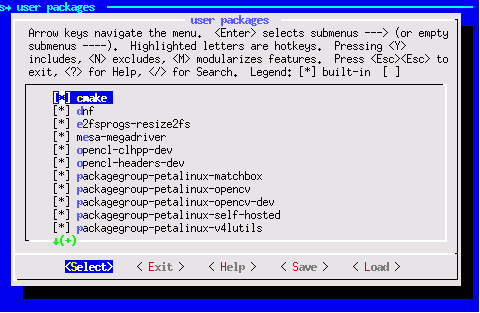
\includegraphics[width=150mm, keepaspectratio]{figures/plnx.png}
    \caption{Petalinux konfigurációs felülete}
\end{figure}

A csomagok hozzáadásán kívül lehetőségünk van a generált device tree módosítására is. Ez főleg saját tervezésű PCB-k esetében fontos, azonban Xilinx által gyártott tesztkártyák esetében is szükséges lehet néhány paraméter módosítása. Ebben a feladatban a generált device tree megfelelt az elvárásoknak, így nem kellett módosítanom rajta.

Végül pedig engedélyezni kellett az ext4 rootfs-t, és a tftpboot-ot. Előbbi azt jelenti, hogy az operációs rendszer boot partíciója lehet ext4 partíció, míg utóbbi azt teszi lehetővé, hogy a boot partíció ne az eszközön, hanem egy távoli tftp (Trivial File Transfer Protocol) szerveren legyen tárolva. Ezen kívül engedélyeznünk kell a NFS (Network File System) használatát is, amivel a rootfs partíció is távoli szerverről lehet elérhető. Ez utóbbi két dolog megkönnyíti a fejlesztés folyamatát, hiszen egy SD kártya írása helyett a kész image-et csak egy szerverre kell másolni, valamint még nagyobb előny, hogy fizikailag nem kell a kártya közelében tartózkodnunk.

Ezután csak ki kell adnunk a \mycode{petalinux-build} parancsot, és elkezdődik a build folyamat. Ennek eredménye egy SD kártyára írható image. Ebben a feladatban az image-et egy szkript segítségével szét kellett bontani a két partícióra, ezeket a szerveren két külön helyre kell majd másolni a helyes működéshez.

\section{Vitis platform}

